\begin{figure}[htp]
\caption{Medienverzicht}\label{fig:AppMedienverzicht}
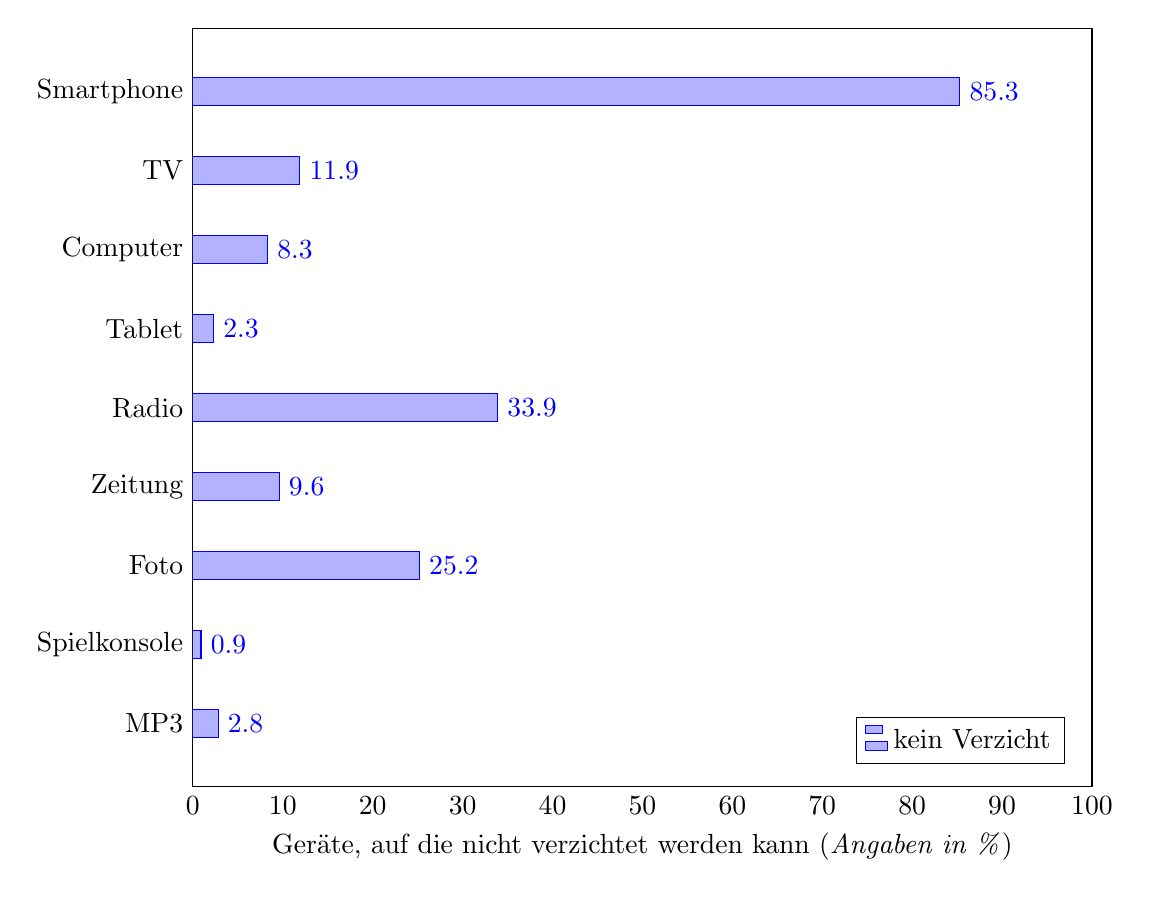
\begin{tikzpicture}[scale=1]
  \begin{axis}[
    xbar,
    %y axis line style = { opacity = 0 },
    %axis x line       = none,
    tickwidth         = 0pt,
    xmin              = 0,
    xmax              = 100,
    %enlarge y limits  = 0.1,
    %enlarge x limits  = 0.02,
    reverse legend,
    legend pos=south east,
    ytick             = data,
    xlabel            = {Geräte, auf die nicht verzichtet werden kann (\textit{Angaben in \%})},
    %height            = 20cm,
    width             = 13cm,
    symbolic y coords = {MP3, Spielkonsole, Foto, Zeitung, Radio, Tablet, Computer, TV, Smartphone},
    nodes near coords,
    nodes near coords align={horizontal},
  ]
  %nicht verzichten
  \addplot coordinates { (85.3,Smartphone)(11.9,TV)(8.3,Computer)(2.3,Tablet)(33.9,Radio)(9.6,Zeitung)(25.2,Foto)(.9,Spielkonsole)(2.8,MP3)};
  
  \legend{kein Verzicht}
  \end{axis}
\end{tikzpicture}
\end{figure}